% Preview source code

%% LyX 2.0.3 created this file.  For more info, see http://www.lyx.org/.
%% Do not edit unless you really know what you are doing.
\documentclass[12pt,twoside,english]{article}
\usepackage[T1]{fontenc}
\usepackage[latin9]{inputenc}
\usepackage[letterpaper]{geometry}
\geometry{verbose,tmargin=1.25in,bmargin=1.25in,lmargin=1.25in,rmargin=1.25in}
\setlength{\parskip}{\bigskipamount}
\setlength{\parindent}{0pt}
\usepackage{color}
\definecolor{note_fontcolor}{rgb}{0.80078125, 0.80078125, 0.80078125}
\usepackage{verbatim}
\usepackage{amsthm}
\usepackage{amsmath}
\usepackage{amssymb}
\usepackage{graphicx}
\usepackage{esint}

\makeatletter

%%%%%%%%%%%%%%%%%%%%%%%%%%%%%% LyX specific LaTeX commands.
%% The greyedout annotation environment
\newenvironment{lyxgreyedout}
  {\textcolor{note_fontcolor}\bgroup\ignorespaces}
  {\ignorespacesafterend\egroup}
%% A simple dot to overcome graphicx limitations
\newcommand{\lyxdot}{.}


%%%%%%%%%%%%%%%%%%%%%%%%%%%%%% User specified LaTeX commands.
\usepackage{mathtools}
\DeclareMathOperator{\Tr}{tr}
\DeclareMathOperator{\Grad}{grad}
\DeclareMathOperator{\Div}{div}
\DeclareMathOperator{\Curl}{curl}
\usepackage{cancel}
\DeclareMathOperator{\re}{Re}
\DeclareMathOperator{\im}{Im}
\usepackage{lipsum}
\usepackage{siunitx}

\makeatother

\usepackage{babel}
\begin{document}

\title{Mapping the North Polar Spur Using the Hydrogen Line}


\author{Caleb Levy \\
\\
with Isaac Domagalski and Aaron Tran}
\maketitle
\begin{abstract}
In this report we 
\end{abstract}
\rule[0.5ex]{1\columnwidth}{1pt}


\section*{Introduction}

One of the most important facts about the baryonic matter in our universe
is that the vast majority of it consists of hydrogen atoms. Hydrogen,
when excited and de-excited, produces very specific sets of emission
and absorbtion lines, giving the emitted light a number of signature
properties. As any large body of matter in our universe can be assumed
to consist mostly of hydrogen, we can use these signature properties
to construct profiles of astronomical objects.

\begin{comment}
One particular form of light from hydrogen is of special interest
to radio astronomers. Separate from the more familiar visible and
ultraviolet photons predominatly found in stars, 
\end{comment}
Of particular interest to radio astronomers is radiation emitted from
the a hyperfine transition of a neutral hydrogen atom. This transition,
known as the hydrogen line, occurs at the $\SI{1420.4058}{\mega\hertz}$
frequency, or $\SI{21}{\centi\meter}$ wavelengths, and arises from
the spin states of the electron and proton falling out of alignment.
Although an extroniarily rare transition for any given hydrogen atom
to undergo, the sheer abundance of neutral hydrogen dictates that
our view of the sky is dominated by the hydrogen line at $\SI{21}{\centi\meter}$
wavelengths.

As seen from the atom's rest frame, hyperfine transitions have very
narrow spreads in frequency. Because of this, we can reconstruct properties
of objects in the sky by analyzing their spectra. Frequency peaks
above $\SI{1420.4}{\mega\hertz}$ correspond to blue-shifts from atoms
moving toward us; peaks below this frequency are redshifts from atoms
moving away. Because neutral hydrogen is optically thin in our galaxy,
it is also possible to map out the three dimensional structure of
astronomical objects by analyzing different peaks originating from
various depths within hydrogen clouds.

In this report we apply the above principals to mapping the structure
of the North Polar Spur. The first three sections outline the overall
process for gathering and preparing data. Section 1 begins with an
introduction to this structure, outlining basic properties and information
which we undertake to investigate. In Section 2, we describe our process
and reasoning for scheduling observations and recording spectra. In
section 3, we discuss the techniques we employed to remove and account
for noise, interference and distortions which arose in our recorded
signals.

The remaining sections summarize the results. In Section 4, we describe
our method of translating spectra into temperature, velocity and column
density measurements. These measurements are used to create 2D color
plots of the velocity and column densities of the North Polar Spur,
which are displayed and analyzed in Section 5. Finally, we offer our
concluding remarks in Section 6. 


\section{Schedule of Observations}

The North Polar Super is a massive collapsed super-nova remnant, composed
of an infalling cloud of gas found at galactic longitudes $\SI{220}{\degree}\le l\le\SI{20}{\degree}$
and latitudes $\SI{0}{\degree}\le b\le\SI{90}{\degree}$,%
\footnote{That is $\SI{220}{\degree}$ to $\SI{380}{\degree}$ modulo $\SI{360}{\degree}$,
or from $\SI{220}{\degree}$ to $\SI{360}{\degree}$ and wrapping
around from $\SI{0}{\degree}$ to $\SI{20}{\degree}$.%
} occupying roughly one quarter of the celestial sphere. However much
of it is in the Southern hemisphere, thus we were only able to see
a portion of this structure. %
\begin{lyxgreyedout}
what can we see? Our axes are labelled to carve out this whole area. %
\end{lyxgreyedout}


For this observation, we employed a $\SI{3.7}{\meter}$ radio dish
located atop Mount Leuchner, located just outside of Berkeley at $\SI{37}{\degree}$
North and $\SI{122}{\degree}$ West. At $\SI{21}{\centi\meter}$ wavelengths,
this telescope possesses a half power beamwidth of $\SI{4}{\degree}$,
making it incapable of perceiving structures with angular radius smaller
than $\SI{4}{\degree}$ on the sky. The Nyquist critereon, as applied
to our object, dictates that we would require telescope pointings
spaced at most $\SI{2}{\degree}$ in each direction to extract all
the information that we can given the limits of our telescope.

In order to map out where to point to on the sky, we created a grid
in $l$ and $b$ with $45$ points in lattitude going from $\SI{0}{\degree}$
to $\SI{90}{\degree}$, achieving the desired spacing of $\SI{2}{\degree}$.
While a change of $\Delta b$ in latitude always corresponds to an
angular motion of $\Delta b$ degrees along the celestial sphere,
the angular distance between two points $\Delta l$ degrees apart
on the sky is latitude dependent, scaling as $\Delta l/\cos b$ for
small $\Delta l$. To account for this, and avoid extraneous telescope
pointings, we spaced points in our grid a distance $\SI{2}{\degree}/\cos b$
for each given $b$. We then added to our list of latitudes corresponding
to each $b$ until either filling out the spatial extent of our object
or reaching one of the telescope pointing limits.

From there we performed a brute force calculation for each coordinate
by checking whether it would be visible during any $15$ minute interval
for the duration of the lab. Those points which we found would be
visible were marked as viewable on our reference grid, and at such
times that we could observe, the telescope was directed to traverse
the grid row by row so as to minimize time spent mechanically moving
the telescope to track the objects. Each night we would update our
grid to check off the new points which had been observed, so that
our tracking software would skip them on the next observation.

Fully imaging the North Polar Spur at this resolution requires roughly
$2500$ pointings; i.e. the full extent of the viewable portion of
the North Polar Spur consists $2500$ pointings on the sky. Of those,
around $1600$ pointings can be made with our telescope at this time
of year, so ideally we would have $1600$ distinct galactic coordinate
values on the sky corresponding to our object.%
\begin{lyxgreyedout}
Here goes picture from Isaac's website if possible.%
\end{lyxgreyedout}
{} Unfortunately, a combination of time mismanagement on the part of
ourselves and other research teams making use of the telescope, hardware
and software problems which prevented use of the telescope on several
occasions, and spurious system errors rendering a portion of our observations
unuseable, we were only able to gather about $450$ useable points
of data.

In order to make best use of the time we had available, we chose to
maximize coverage of the sky as opposed to taking detailed images
of any given area. Our data thus covers most of the North Polar Spur's
angular extent. Due to the sparsity of points our image is less detailed
than desireable, and perhaps more importantly, is more difficult to
use for visually removing outlier points from our data, as each point
constitutes a greater portion of our image than if we had more tightly
spaced data. Despite this, we have good reason to believe that our
image is accurate. We describe our analysis in Sections 4 and 5.


\section{Recording Spectra}

The hydrogen line occurs at a frequency of $\SI{1420.4}{\mega\hertz}$.
In order to record this, the raw signal from the dish was mixed with
a local oscillator running at $1270.4\pm\SI{1.5}{\mega\hertz}$, and
then run through a filter to remove the additive components, placing
line center at roughly $\SI{150}{\mega\hertz}$. The raw data from
the ADC was then processed by an FPGA which performed real time fourier
transforms to return the power spectrum of the input signal over the
IF range of $144-\SI{156}{\mega\hertz}$, divided into $8192$ bins,
giving us a frequency window of $\SI{12}{\mega\hertz}$ about line
center with a frequency resolution of $\SI{1.5}{\kilo\hertz}$. 

There is no source within our galaxy that we have reason to believe
would be moving toward or away from us with speed greater than $\SI{250}{\kilo\meter\per\second}$.
Using the Doppler shift formula for light, this is equavlent to saying
$\left|\Delta f_{\textnormal{Doppler}}/f_{\textnormal{H line}}\right|\lesssim8.3\times10^{-4}$,
meaning we should see no spectra shifted more than $\SI{1.2}{\mega\hertz}$
from line center. We thus required a minimum of $\SI{3}{\mega\hertz}$
of bandwidth about line center in order to ensure that we capture
all relavent parts of our signal.

In order remove the shape of the bandpass filter from our measurements,
we recorded spectra with the local oscillator frequency shifted both
$\SI{1.5}{\mega\hertz}$ above and below line center. This allowed
us to obtain the shape of the bandpass unmodified by the hydrogen
spectrum on each side. We used to divide out the noise in the manner
described in the next section. 

Performing this analysis required that the full frequency window of
interest be contained in both the right and left-shifted spectra,
and simultaneously that these two spectra do not overlap on the frequency
ranges we wanted to examine. Combining these requirements with the
fact that the $\SI{1}{\mega\hertz}$ boarder on each side of our spectra
were unusable due to the presence of the bandpass filter was what
resulted in the choice of a $\SI{12}{\mega\hertz}$ bandpass.

\begin{comment}
Although a higher sampling rate could yield more precise spectral
measurements, a frequency window of $\SI{12}{\mega\hertz}$ about
line center was chosen to optimize our spectral resolution while retaining
the ability to normalize our spectra to an absolute temperature in
the sky.
\end{comment}
\begin{comment}
Performing the normalization 

as the of frequency window outlined in Figure .
\end{comment}
To determine our sampling time, we noted that the average kinetic
temperature of the hydrogen atoms in these clouds is on the order
of $\SI{100}{\kelvin}$. Making use of the eponymous shorthand for
the kinetic energy of a typical atom, given by 
\[
\frac{1}{2}m_{\textnormal{H}}\left\langle v_{\textnormal{thermal}}^{2}\right\rangle =k_{b}T,
\]
and plugging in the appropriate parameters yiels a thermal velocity
of order $\SI{2}{\kilo\meter\per\second}$, meaning we should expect
fluctuations in the frequency of the spectra on the order $\SI{15}{\kilo\hertz}$.
Allowing for a factor of ten safety margin in our estimates of these
fluctuations yields the $\SI{1.5}{\kilo\hertz}$ frequency resolution
used for our observations.



Prior to processing, the raw data output from the FPGA contains substantial
amounts of noise, distortion, and artifacts, the causes of which are
detailed in Figure . Any single recorded spectra is unuseable due
to this noise. However, using the central limit theorem as guidance
and assuming that the noise is in fact random, we can conclude that
averaging many spectra together will tend to average out the noise
and recover the desired signal. 

Through some experimentation we determined that an average of about
two minutes per pointing was adequate to recovering our signal. Of
this, one minute was spent recording the left-shifted LO frequency
offset, and one minute on the right-shifted offset. Additionally,
for both of these offsets, we recorded for five seconds with the equivalent
of a $\SI{100}{\kelvin}$ blackbody's spectrum injected into the signal
via a noise diode to be used for calibrating the light temperature
of our hydrogen cloud. 

The shape of the bandpass filter changes slowly over time, thus for
each pointing we recorded, in order: left-shifted spectra, left-shifted
calibration spectra, right-shifted calibration spectra and the right-shifted
spectrum. This ensured that our noise measurements were equidistant
in time from both of their respective sets of data.

\begin{figure}
\caption{\label{fig:Sources of Noise}}
\end{figure}



\section{Smoothing and Calibration}


\subsection{Removal of RF Spikes}

One of the first problems we were required to deal with when calibrating
our data were major RF spikes from overhead airplanes, depicted in
Figure . In order to deal with this, we used a ``minimum smoothing''
method. In order to get rid of the RF spikes, we divided the 8192
data points in our spectra into 2048 sequential bins of four elements,
took the minimum element in each bin, recordeding the index of that
element in the original array. We then made an array of those points,
and recorded the frequencies corresponding to the indices of the array.

There are several potential drawbacks to using this method. Any downward
signal spikes in our data will make it into the filtered array; if
these spikes are located far off line-center, they could heavily distort
our derived velocity measurements since they will be used as weights
for very high velocities. This method depends on there being a well
defined underlying profile (well-defined bandpass shape). It also
runs the risk of systematically underestimating the strength of the
signal, since we are biasing toward the minimum. 

There is a possibility of removing imortant information about the
spectral profile from our data, since we are throwing out 3/4 of our
data points. Finally, if the frequencies of the RF spikes are constant
in time, we run the risk of inducing a small but systematic shift
in the measured frequency of our line spectra.

In practice, after examining large numbers of our spectra, we concluded
that this method worked very well. Emperically there is a very well
defined shape for the signal from this telescope, and there are very
few downward spikes in our data. Even if there is a systematic frequency
offset in our data, there error will be of order at most $\SI{10}{\kilo\hertz}$,
around $1\%$ of the typically expected Doppler shifts in our frequency
data. The effect is thus likely minimal.


\subsection{Calibration of Temperatures}

In order to determine the physical brightness temperature of our hydrogen
clouds, we need to understand the various sources of noise and distortion
in our system and sequentially eliminate them. 

At the antenna itself, there are two primary sources from which our
signal originates: the light from the hydrogen cloud which is at light
temperature $T_{\textnormal{sky}}$, and the radiation from the telescope
itself, which given our narrow frequency band can be roughly treated
as a blackbody emitting radiation at a temperature $T_{\textnormal{sys}}$.
\begin{lyxgreyedout}
Is this accurate?%
\end{lyxgreyedout}
{} The signal originating from the telescope can be viewed as a power
spectrum emitted from a source with temperature $T_{\textnormal{sys}}+T_{\textnormal{sky}}\left(\nu\right)$. 

This signal is passed through a number of amplifiers which multiply
the entire signal by a gain factor whose value is constant in frequency,
or channel number %
\begin{lyxgreyedout}
Need I define this?%
\end{lyxgreyedout}
. Ideally, our gain factors would remain the same for each pointing,
however due to equipment problems we consistently measured different
gains $g_{\textnormal{left}}$ and $g_{\textnormal{right}}$ when
raising and lowering the local oscillator frequency.%
\footnote{Here $g_{\textnormal{left}}$ refers to the gain when our spectra
was shifted left of center and $g_{\textnormal{right}}$ refers to
the signal shifted right of center.%
} These gain factors also shift our temperature measurement into arbitrary
units whose values we must calibrate. Finally, the overall shape of
our signal is modulated by the bandpass function $\beta\left(\nu\right)$
whose profile is a strict function of channel number. The signals
we recieve are thus given by 
\begin{align*}
S_{\textnormal{left}} & =g_{\textnormal{left}}\beta\left(\nu\right)\left(T_{\textnormal{sys, left}}+T_{\textnormal{sky}}\left(\nu\right)\right)\\
S_{\textnormal{right}} & =g_{\textnormal{right}}\beta\left(\nu\right)\left(T_{\textnormal{sys, right}}+T_{\textnormal{sky}}\left(\nu\right)\right).
\end{align*}


First, we use our noise measurements to interpret our signal in units
of Kelvin. Clipping off the outer parts of our frequency spectra at
the edges of our bandpass filter, and excising the respective portions
of our power spectra containing contributions from $T_{\textnormal{sky}}$,
we sum over all points in our array with noise and without, to obtain
that 
\begin{align*}
Y_{\textnormal{left}}\equiv\frac{\sum S_{\textnormal{left cal},i}}{\sum S_{\textnormal{left},i}} & =\frac{\sum g_{\textnormal{left}}\beta_{i}\left(T_{\textnormal{sys, left}}+T_{\textnormal{noise}}\right)}{\sum g_{\textnormal{left}}\beta_{i}T_{\textnormal{sys, left}}}\approx\left(\frac{T_{\textnormal{noise }}}{T_{\textnormal{sys, left}}}+1\right)\\
\implies T_{\textnormal{sys, left}} & =\frac{T_{\textnormal{noise}}}{Y_{\textnormal{left}}-1}=\frac{\SI{100}{\kelvin}}{Y_{\textnormal{left}}-1},
\end{align*}
with an identical equation holding for $T_{\textnormal{sys, right}}$.
Here the subscripted quantities denote values which depend on channel
number.

Our gain factors are different for both the left and right shifted
spectra, however we only care about their ratio. To find this, we
excise any points in our array lining up with channel numbers which
have contributions from hydrogen emission. Our gain ratio is thus
defined by 
\[
R_{g}=\frac{\sum S_{\textnormal{right},i}}{\sum S_{\textnormal{left},i}},
\]
where again the sum is taken over the indices corresponding to frequency
channels containing neither right-shifted nor left shifted radiation
from the hydrogen line, as depicted in Figure \ref{fig:Gain ratio schematic}.

\begin{figure}
\noindent \begin{centering}
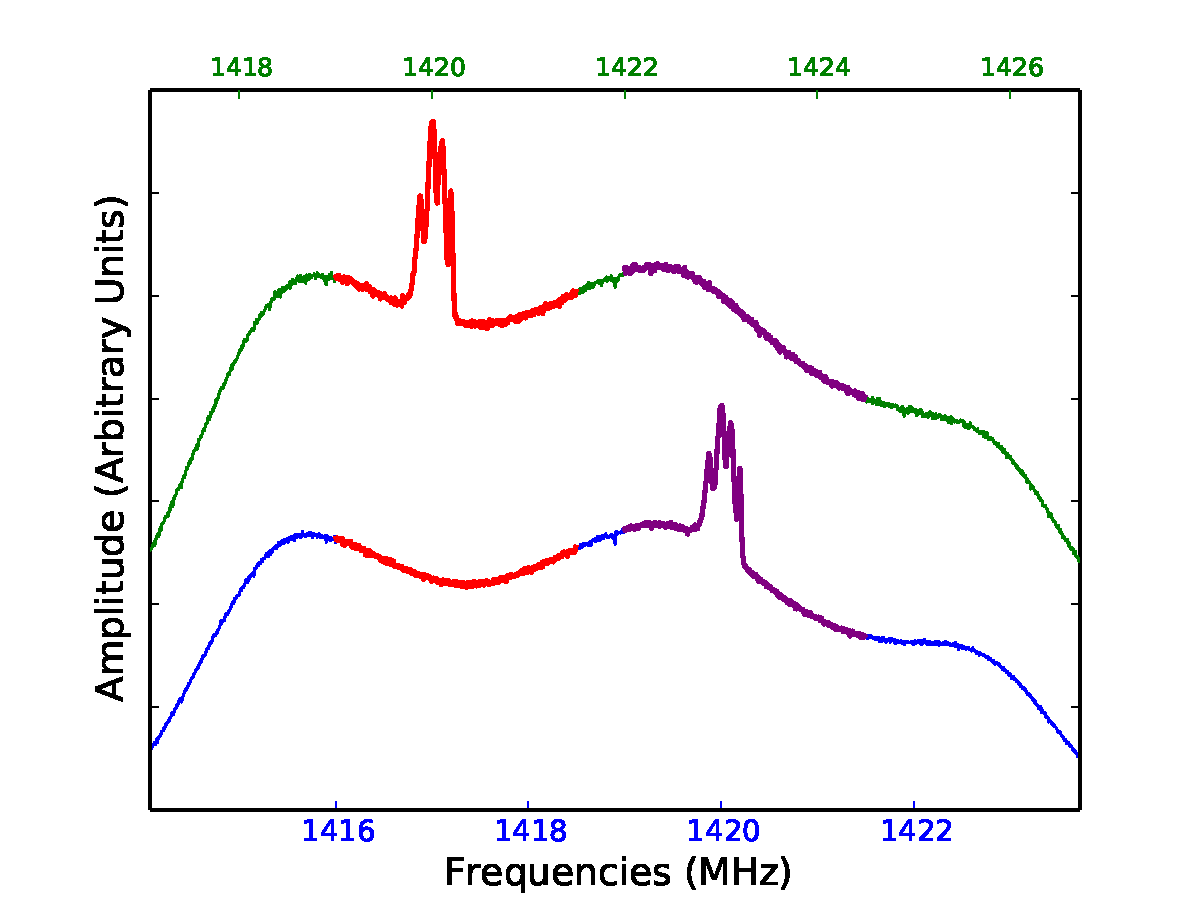
\includegraphics[width=5in]{\lyxdot \lyxdot /\lyxdot \lyxdot /\lyxdot \lyxdot /galaxy-lab/langley/image-files/Excized_Regions}\caption{Schematic of the excized regions of our hydrogen emission spectra.
The red region is removed when normalizing temperatures for the left-shifted
spectra; the purple is removed when finding the sky temperatures for
the right-shifted spectra. Only the blue and green regions are used
when finding the gain ratio between the two spectra.\label{fig:Gain ratio schematic}}

\par\end{centering}

\end{figure}

\end{document}
